\chapter[Appendix 4b (supplementary to Chapter 4)]{Appendix 4b (supplementary to Chapter 4)}

\begin{landscape}
\begin{figure}[h!]
\begin{center}
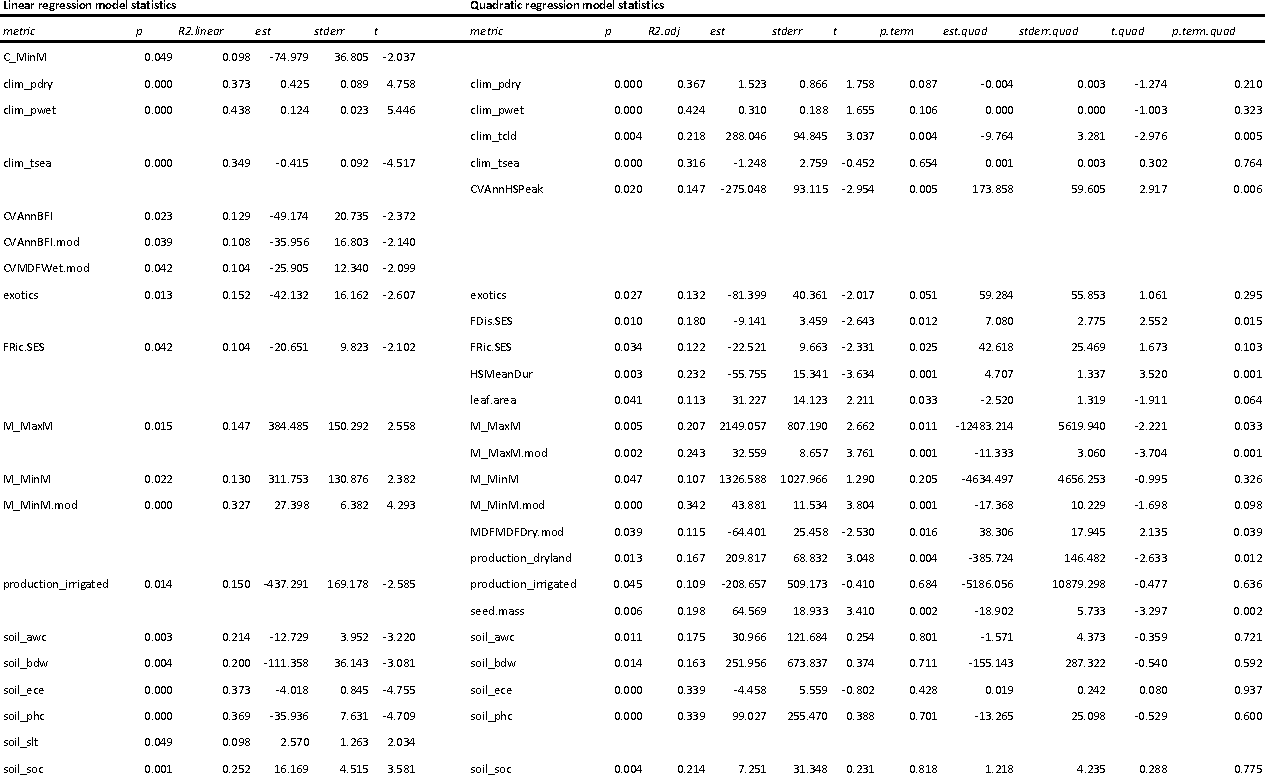
\includegraphics[width=20cm]{regression_stats_sprichChao1.pdf} % figures can be in pdf, png, jpeg or eps format
\caption[Univariate OLS regression statistics for species richness.]{\small{Univariate OLS regression statistics for species richness.}} %The caption in the square bracket is used for the table of figures. The caption in the curved brackets is the one that is printed as actual caption. 
\label{fig:Ch4sup2_F1} % label for cross-referencing
\end{center}
\end{figure}   
\end{landscape}
\clearpage

\begin{landscape}
\begin{figure}[h!]
\begin{center}
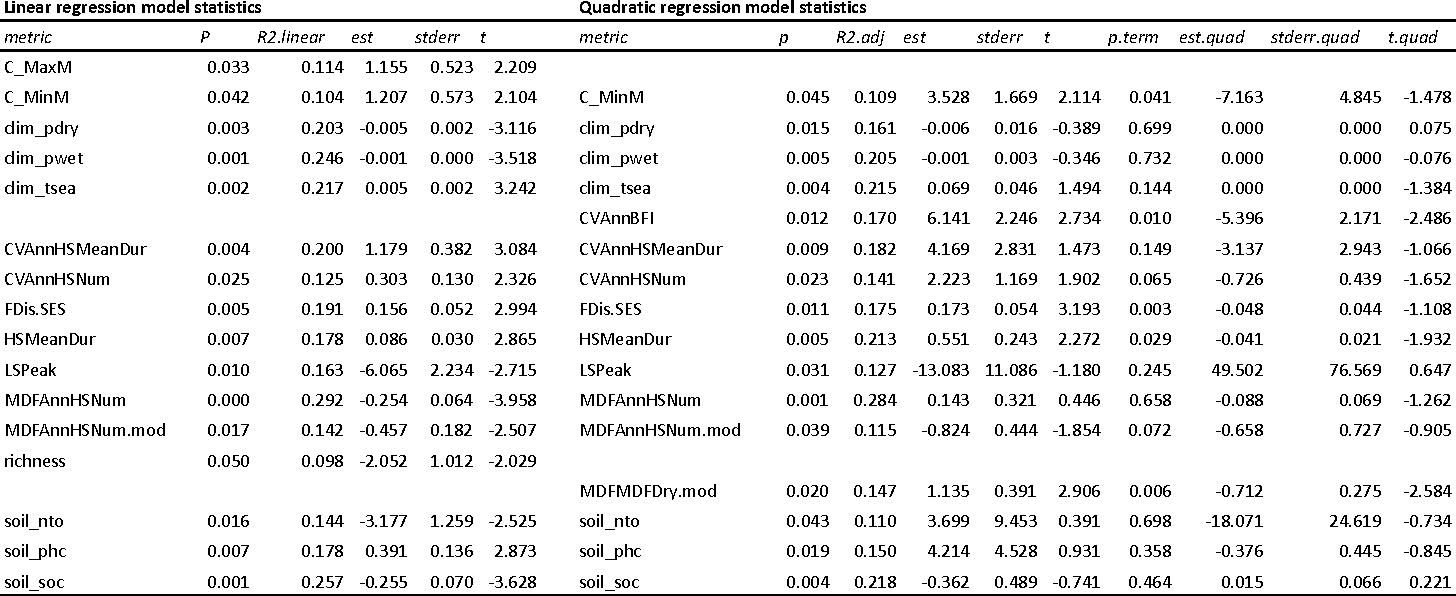
\includegraphics[width=20cm]{S2b.pdf} % figures can be in pdf, png, jpeg or eps format
\caption[Univariate OLS regression statistics for FRic.SES.]{\small{Univariate OLS regression statistics for FRic.SES.}} %The caption in the square bracket is used for the table of figures. The caption in the curved brackets is the one that is printed as actual caption. 
\label{fig:Ch4sup2_F1} % label for cross-referencing
\end{center}
\end{figure}   
\end{landscape}
\clearpage

\begin{landscape}
\begin{figure}[h!]
\begin{center}
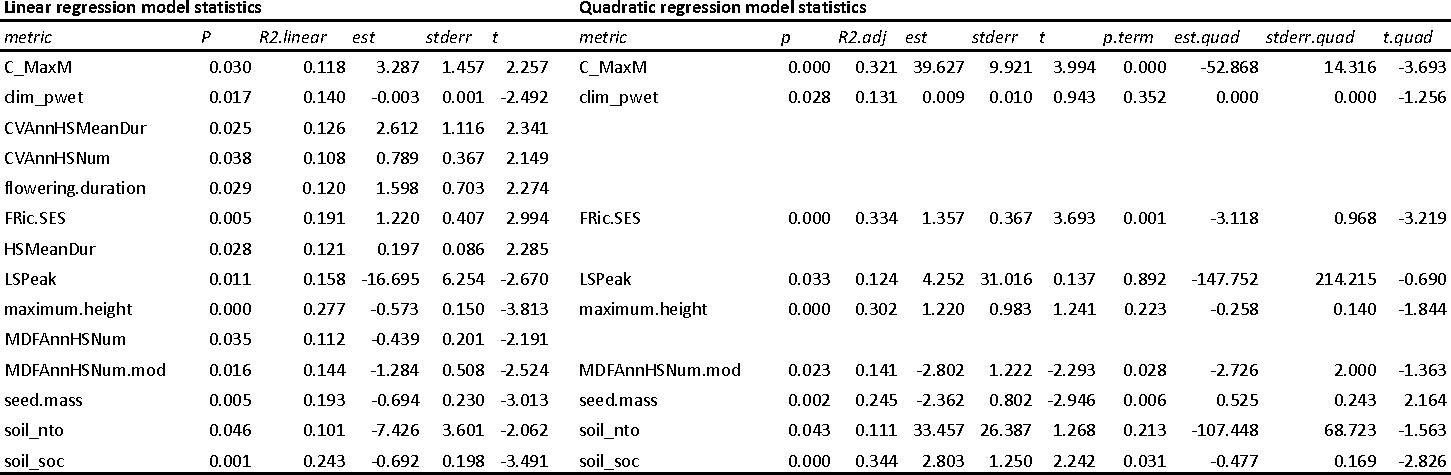
\includegraphics[width=20cm]{S2c.pdf} % figures can be in pdf, png, jpeg or eps format
\caption[Univariate OLS regression statistics for FDis.SES.]{\small{Univariate OLS regression statistics for FDis.SES.}} %The caption in the square bracket is used for the table of figures. The caption in the curved brackets is the one that is printed as actual caption. 
\label{fig:Ch4sup2_F1} % label for cross-referencing
\end{center}
\end{figure}   
\end{landscape}
\clearpage

\begin{landscape}
\begin{figure}[h!]
\begin{center}
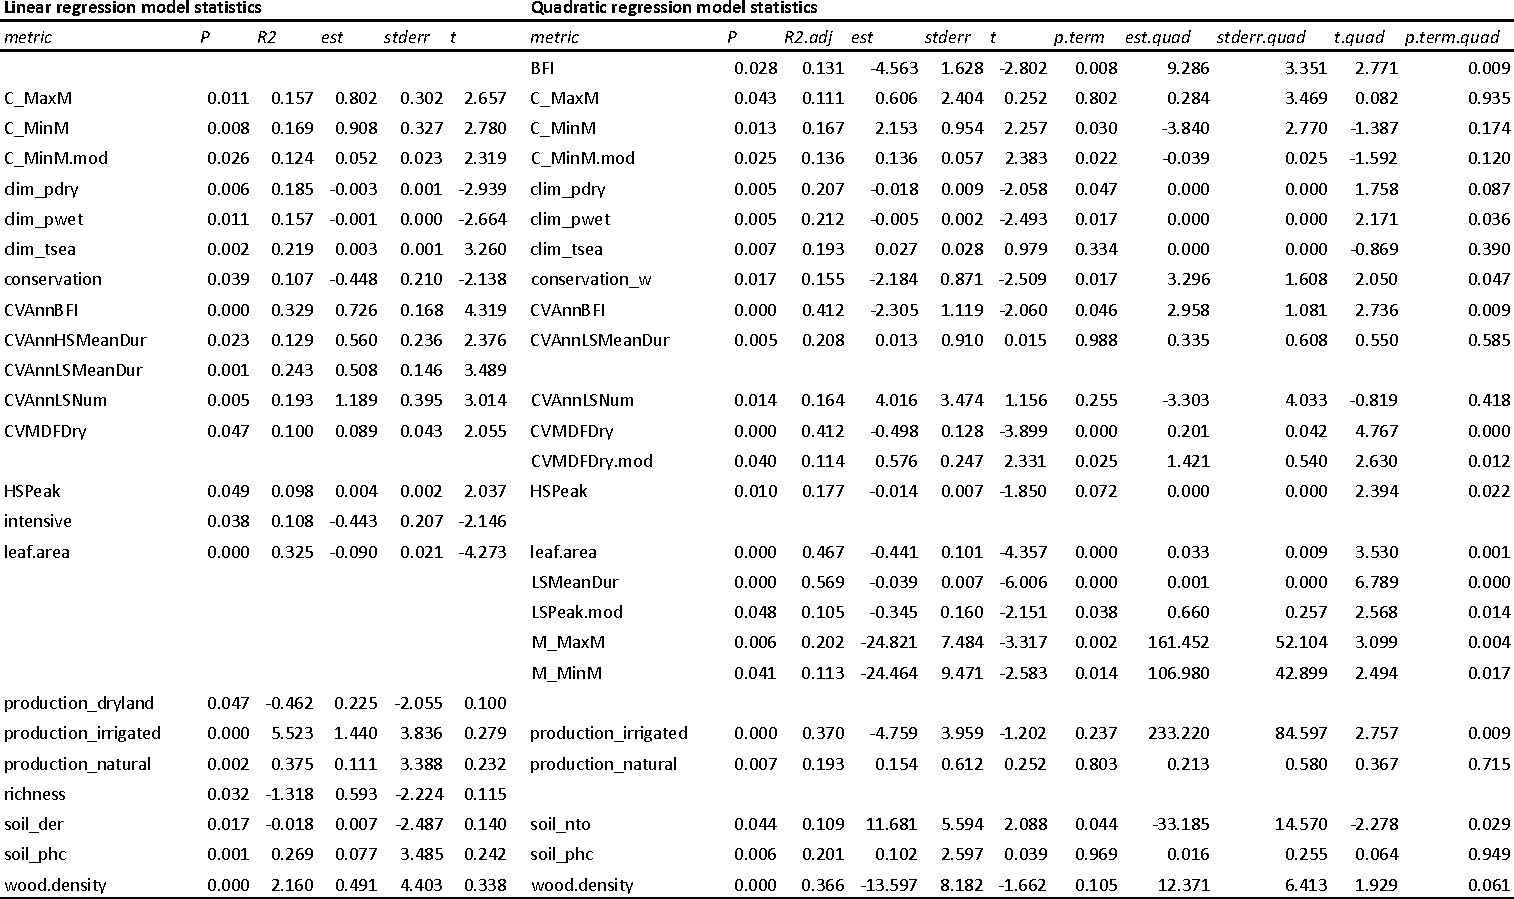
\includegraphics[width=20cm]{S2d.pdf} % figures can be in pdf, png, jpeg or eps format
\caption[Univariate OLS regression statistics for exotic abundance.]{\small{Univariate OLS regression statistics for exotic abundance.}} %The caption in the square bracket is used for the table of figures. The caption in the curved brackets is the one that is printed as actual caption. 
\label{fig:Ch4sup2_F1} % label for cross-referencing
\end{center}
\end{figure}   
\end{landscape}
\clearpage

